\documentclass{article}
\usepackage{amssymb}
\usepackage{amsmath}
\usepackage{fancyhdr}
\usepackage{harvard}
\usepackage[hidelinks]{hyperref}
\citationmode{abbr}
\citationstyle{dcu}
\pagestyle{fancy}
\usepackage{graphicx}
\graphicspath{ {images/} }
\lhead{Justin Coker | Problem Set 4}
\rhead{}
\begin{document}
Estimating the following model:

$$f(b, t) = Stations * Pop + \alpha Corp * Pop + \beta Dist  + \epsilon$$

To examine the impact of corporate ownership and distance on radio station mergers.

Following Akkus, Cookson, and Horta\c csu (2016) using the maximum score estimator:

$$\beta = \text{argmax} Q(\beta) = \sum_{y=1}^{2} \sum_{b = 1}^{M_y -1}\sum_{b^\prime = b+1}^{M_y} 1[f(b, t|\beta) + f(b^\prime, t^\prime|\beta) \geq f(b^\prime, t|\beta) + f(b, t^\prime|\beta)]$$

To do so, I create a two payoff matrices one for actual matches and counter-factual matches.

The payoff matrix for actual matches is simply an M X 1 vector where M is the number of buyer/target matches in a given year. The counter-factual pay-off matrix is M x (M-1) where the elements are as below:

$$(i, j) \text{ element} = \begin{cases} \text{f(buyer i, target (j+1))}, & \mbox{if } j < (i - 1) \text{ or } i = M\\ \text{f(buyer i, target (j + 2))}, & \text{otherwise} \end{cases}$$ 

I use list comprehension in python (due to its speed relative to standard for loops) to create and evaluate these matrices during the optimization process (see max\_ score.py and payoff\_ func.py)

After transforming price and population into hundreds of thousands of people and dollars, I receive the following results from this estimation (See Results 1 section below):

$$f(b, t) = Corp * Pop + 274.77 * Stations * Pop + -2.33 * Dist  + \epsilon$$
using Differential Evolution method, and

$$f(b, t) = Corp * Pop + 277.5 * Stations * Pop + -2.3 * Dist  + \epsilon$$

using Nelder-Mead method.
\newpage

Note that the Nelder-Mead is particularly sensitive to the initial guess. The initial guess I used is $\alpha = 300$ and $\beta = -2$. These guesses were derived from results of the differential evolution method using fairly wide bounds.\\


The differential evolution method is quite inconsistent here, especially in the estimation of alpha (see Results 1a below). I contend this is because the variable Corp\_ Owner\_ Buyer has very little variation. In fact, only 2 buyers across all years have a non-zero value for this variable. Therefore, $\alpha$ has very little impact on the value of the equation, leading the optimizer to these shaky results.\\

As such, I hesitate to give much interpretative power to the magnitude of this estimate. Its sign does appear to be consistently positive (even when extending the bounds into the negative quadrant) so I am comfortable stating that corporate ownership appears to increase the desired post merger size (stations * population) of a potential merger.

The coefficient estimated for Distance is much more consistent, even when extending its bounds. It appears that an increase in distance of 1 mile decreases the desired post merger size by about 200,000. \\
\\

To identify target specific characteristics, we must use a slightly different estimator. To estimate the following equation:

$$f(b, t) = \delta Stations * Pop + \alpha Corp * Pop + \gamma HHI + \beta Dist  + \epsilon$$

we use the following:
$$\beta = \text{argmax} Q(\beta) = \sum_{y=1}^{2} \sum_{b = 1}^{M_y -1}\sum_{b^\prime = b+1}^{M_y} 1[f(b, t|\beta) - f(b, t^\prime|\beta) \geq p_{bt} - p_{b^\prime t^\prime} \text{ \& } f(b^\prime, t^\prime|\beta) - f(b^\prime, t|\beta) \geq p_{bt} - p_{b^\prime t^\prime}]$$

In doing so, I find the following results:

$$f(b, t) = 619.31 * Stations * Pop + 149.46 * Corp * Pop - 57.60 * HHI - 446.8 * Dist  + \epsilon$$

I again find some consistency issues here, refer to my above comments regarding the Corp variable. Taking these estimates at face value, we again find that corporate ownership increases the desired post merger size and distance reduces it. The new coefficient here is $\gamma$, which illustrates that a higher degree of concentration in the target market reduces the desired post merger size.\\

The coefficient estimates on Distance is not incredibly different (after normalization of $\delta$) from the previous specification. However, the coefficient on $\alpha$ is very different in absolute and relative magnitude. As noted above, these results seem to be inconsistently estimating this coefficient due to the lack of variation in Corp variable.\\

See results 2 section for estimation output.


\newpage
\section*{Results 1.}
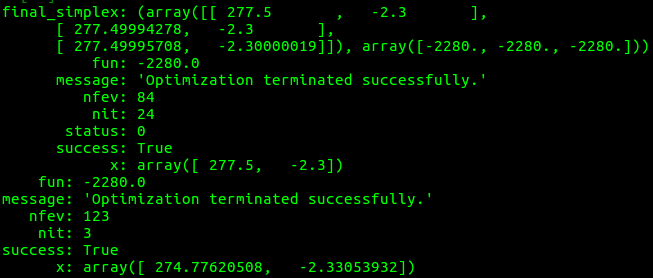
\includegraphics[scale = .65]{Results1}

\newpage
\section*{Results 1a.}
Below we see the results from 4 consecutive estimations. Note that the minimized function value does not change, but the estimate of alpha changes greatly.\\


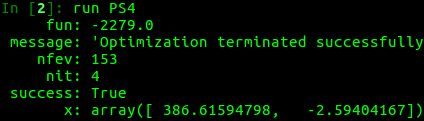
\includegraphics[scale = .65]{Results1A_1}\\

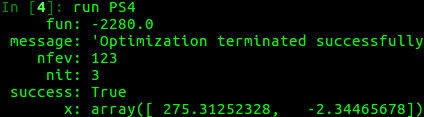
\includegraphics[scale = .65]{Results1A_2}\\

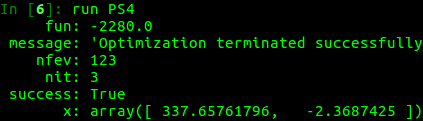
\includegraphics[scale = .65]{Results1A_3}\\

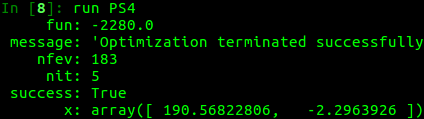
\includegraphics[scale = .65]{Results1A_4}\\

\newpage

\section*{Results 2.}

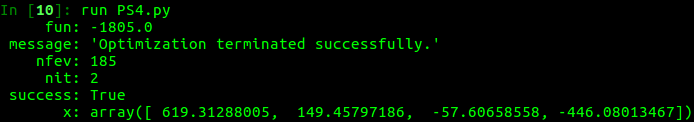
\includegraphics[scale = .65]{Results2}

\end{document}